\documentclass[UTF8]{ctexart}

\usepackage[backend=bibtex]{biblatex}
\usepackage{mathtools}
\usepackage[CJKbookmarks=true,colorlinks,linkcolor=blue,anchorcolor=blue,citecolor=green]{hyperref}
\usepackage{color}
\usepackage{graphicx}
\usepackage{enumerate}
\usepackage{titlesec}
\usepackage{titletoc}
\usepackage{bm}
\usepackage{bbm}
\usepackage{amssymb}

\newcommand{\HRule}{\rule{\linewidth}{0.5mm}}
\newcommand{\myFunc}{}
\newenvironment{myquote}
  {\begin{quote}\kaishu\zihao{-5}}
  {\end{quote}}

\titlecontents{section}
              [0em]
              {\bf \small}%
              {\contentslabel{2.5em}}%
              {}%
              {\titlerule*[0.5pc]{$\cdot$}\contentspage}%

\begin{document}
\begin{titlepage}
\begin{center}

\includegraphics[width=\textwidth]{UESTC-Logo}\\[2cm]
\textsc{\LARGE 计算机学院~$\bullet$~人工智能应用与挑战课程~}\\[1.5cm]
\HRule \\[0.4cm]
{ \huge \bfseries Northeastern SMILE Lab - Recognizing Faces in the Wild项目结题报告\\[0.4cm] }

\HRule \\[1.5cm]
\noindent
\emph{组名}:\quad
\quad {\bf Honkai StarRail}\\
\emph{作者}:\quad
\quad {\bf 刘*}\footnotemark
\quad {\bf 赵**}\footnotemark
\quad {\bf 武**}\footnotemark\\
\emph{指导老师}:\quad
\quad {\bf 文泉}
\end{center}
\footnotetext[1]{电子科技大学计算机科学与工程学院数字媒体技术专业,学号:2022**}
\footnotetext[2]{电子科技大学计算机科学与工程学院数字媒体技术专业,学号:2022**}
\footnotetext[3]{电子科技大学计算机科学与工程学院计算机科学与技术专业,学号:2022**}
\end{titlepage}

\tableofcontents
\newpage

\section{前言}
本篇报告为计算机学院~$\bullet$~人工智能应用与挑战课程~,Honkai StarRail小组的项目结题报告,小组选题为“Northeastern SMILE Lab - Recognizing Faces in the Wild”,(详见网址:\href{https://www.kaggle.com/competitions/recognizing-faces-in-the-wild}{小组选题})。

本篇报告包括项目概况介绍、项目结题完成情况、结题后拟改进措施、参与项目体会、意见与建议五部分。
\section{题目概况}
\subsection{竞赛概况}
我们的选题名为“Northeastern SMILE Lab - Recognizing Faces in the Wild”:基于人脸识别的血缘关系鉴定模型(图:$\left(\ref{fig:competition}\right)$)。本次竞赛的主办方为东北大学的微笑实验室\footnote{Northeastern SMILE Lab},该实验室的研究课题有"Effects of Speech Modification Strategies on Vowel Acoustics for Adolescents with Cerebral Palsy"、"Development of Auditory-Perceptual Speech Features in Preschoolers with Typical Development"、"Innovations in the Evaluation and Management of Pediatric Dysarthria"等\footnote{详见东北大学微笑实验室网址:https://smilelab.sites.northeastern.edu}。

\begin{figure}[!ht]
  \centering
  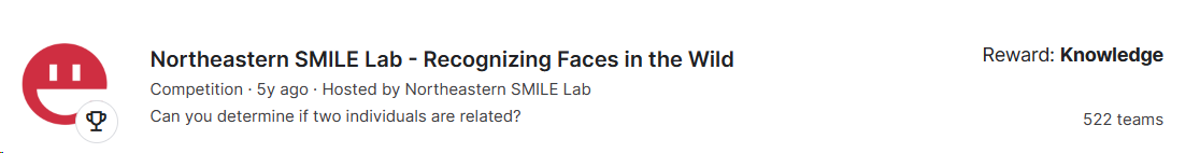
\includegraphics[width=1\textwidth]{competition.png}
  \caption{竞赛题目}
  \label{fig:competition}
\end{figure}

该竞赛的开始时间为2019年5月14日,结束时间为2019年8月9日,竞赛类型为playground。虽然本次竞赛没有实物奖励,但由于该竞赛的题目较有意思,吸引了522支队伍、573位选手参加该竞赛。

\subsection{竞赛内容}
在该竞赛中,题目要求参赛者训练一个模型图像识别模型,该模型能仅通过图像鉴定两人是否有血缘关系。由于用于亲属识别任务的现有图像数据库规模不足以捕捉和反映世界各地家庭的真实数据分布,并且许多隐藏因素会影响家族面部关系,因此需要比计算机视觉算法更有区分度的模型,这也是本竞赛被提出的原因。

由于该竞赛考察的是参赛者模型的识别正确率,故该竞赛的评分标准为\[Score=\frac{N}{M}\],其中N为正确识别血缘关系的测试集数量,M为测试集总数。排行榜也是依据参赛者模型的识别正确率进行排名。

\subsection{竞赛意义}
当今社会,血缘关系鉴定有着多方面、多维度的社会意义:
\begin{itemize}
  \item 当家庭中存在怀疑亲子关系的情况时,血缘关系鉴定有助于维护家庭的稳定与和谐。
  \item 当在法律上出现亲子权纠纷、抚养权争议等问题时,血缘关系鉴定有利于保障当事人的合法权益。
  \item 当对某些人的身份存疑时,如失踪人员寻亲、被拐卖儿童寻亲等,血缘关系鉴定可帮助确认个人身份与亲属关系。
  \item 在医学上可以帮助研究家族遗传病的遗传模式、基因突变的传播等,辅助控制家族遗传病的产生。
\end{itemize}

而现如今最常用的血缘鉴定方式为依据遗传学的基本原理,采用现代化的DNA分型检测技术来综合评判争议个体之间是否存在亲生、隔代或其他血缘关系\footnote{详见https://baike.120ask.com/art/50356}。这种血缘关系鉴定需提取被鉴定者的DNA样本,并通过PCR扩增、后PCR反应、毛细管测序仪检测等步骤完成血缘鉴定,鉴定过程较为繁琐。若能开发出一套基于被鉴定者的外貌特征而实现的亲子鉴定系统,则将大大提高血缘鉴定的效率,减少血缘鉴定的成本。

\subsection{数据规模}
\subsubsection{数据集}
官方给出的测试数据共包含12个文件(详见图$\left(\ref{fig:training data}\right)$),

\begin{figure}[!ht]
  \centering
  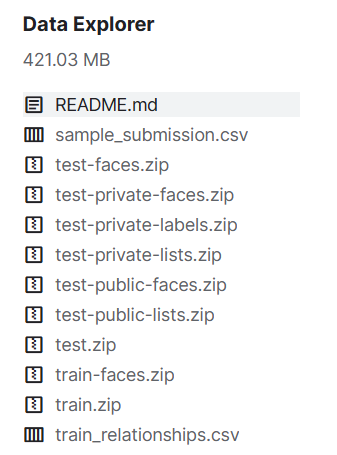
\includegraphics[width=0.5\textwidth]{training data.jpg}
  \caption{测试文件}
  \label{fig:training data}
\end{figure}
其中较为重要的分别是:
\begin{itemize}
  \item train.zip,该文件为所有用于训练的人像图片。
  \item test.zip,该文件为所有用于测试的人像图片。
  \item train\_relationships.csv,该文件中包含了所有含有血缘关系的图片标记,不在这个文件中的图片不含有血缘关系。
  \item sample\underline{\space}submission.csv,该文件为一个正确格式的示例提交文件。列\\
  img\underline{\space}pair描述了图像对,即abcd-efgh表示图像对abcd.jpg和efgh.jpg。\\
  我们的目标是预测test-faces中每对图像是否相关,其中1表示相关,0表示不相关。
\end{itemize}

以上数据文件总大小为421.03MB。

\subsubsection{提交格式} 
在该竞赛中,要求的提交格式如图$\left(\ref{fig:submission}\right)$:
\begin{figure}[!ht]
  \centering
  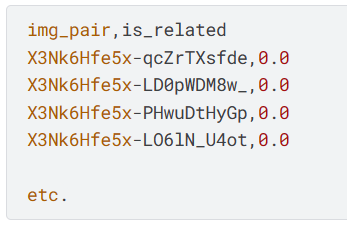
\includegraphics[width=0.5\textwidth]{submission.png}
  \caption{提交格式}
  \label{fig:submission}
\end{figure}

其中img\_pair为测试集中的图像对,图像对中有需要判断是否存在血缘关系的两张图片,is\_related则表示该图像对中的两人是否存在血缘关系,是为1,否为0。在官方给出的提交样例文件sample\underline{\space}submission.csv中,我们可以看到img\_pair与is\_related两个列向量的具体值,如图$\left(\ref{fig:sample}\right)$
\begin{figure}[!ht]
  \centering
  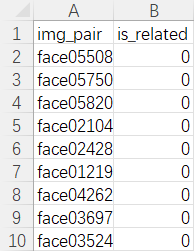
\includegraphics[width=0.5\textwidth]{sample.png}
  \caption{提交样例}
  \label{fig:sample}
\end{figure}

但在我们实际的提交过程中发现,列向量is\_related的数值可以不为0或1,若其值为img\_pair图像对具有血缘关系的可能性,这一文件也是可以被正确提交的,如图$\left(\ref{fig:mysubmission}\right)$
\begin{figure}[!ht]
  \centering
  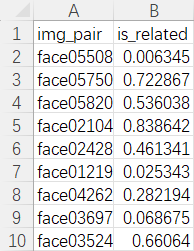
\includegraphics[width=0.5\textwidth]{mysubmission.png}
  \caption{实际提交文件}
  \label{fig:mysubmission}
\end{figure}

\subsection{现有结果}
\begin{figure}[!ht]
  \centering
  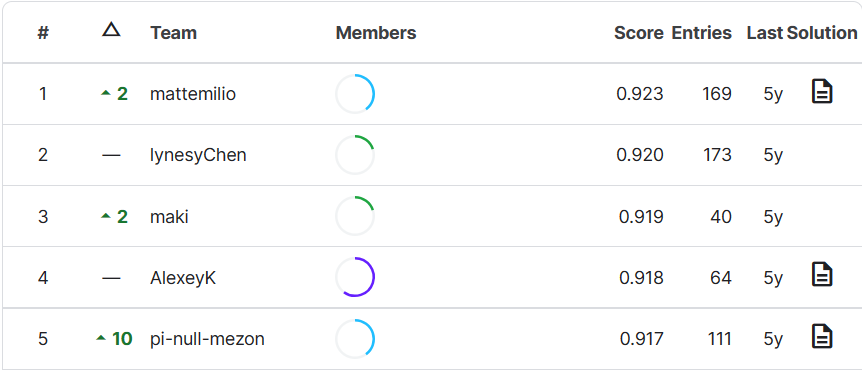
\includegraphics[width=0.7\textwidth]{leaderboard.jpg}
  \caption{排行榜1-5名}
  \label{fig:leaderboard}
\end{figure}
截至目前,共有573位参赛选手,522支参赛队伍。由于该题在五年前已完赛,故参赛选手的最终提交时间均在五年之前。

在该题目的leaderboard中(见图$\left(\ref{fig:leaderboard}\right)$),目前的世界第一为mattemilio,其得分为0.923分,前五名得分均在0.917之上,前一百名得分均在0.894之上。他们的模型识别正确率均能达到九成左右。

\section{项目结题完成情况}
\subsection{当前排名与结果}
本小组最终提交的结果在Private测试集上的得分为0.918, 排名第5;在Public测试集上的得分为0.914, 排名第6。
\begin{figure}[!ht]
    \centering
    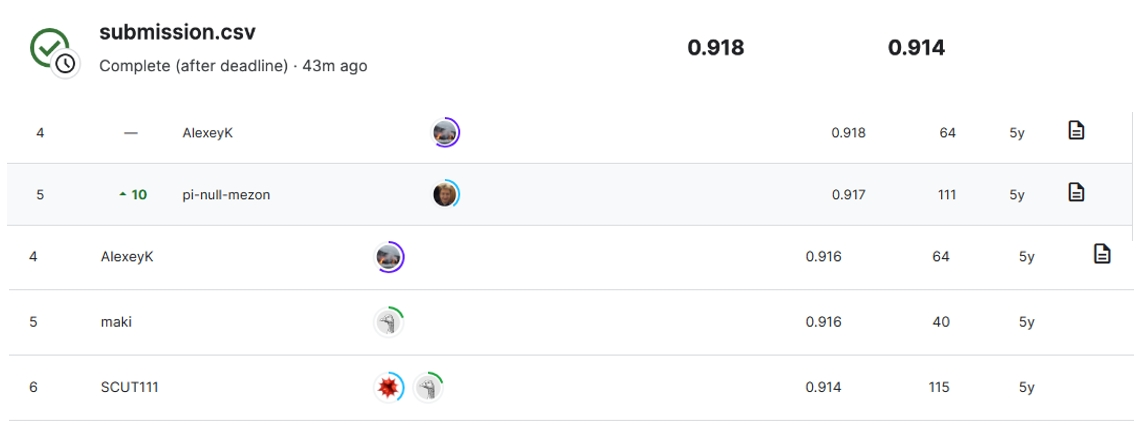
\includegraphics[width=0.7\textwidth]{score.png}
    \caption{最终排名与结果}
    \label{fig:score}
\end{figure}

\subsection{结题模型设计}
\subsubsection{开题设计}
我们开题时使用的模型为Google开发的用于人脸识别与人脸验证的FaceNet,它能够将输入的人脸图像转换为一个128维的向量,被称为人脸嵌入(face embedding),其中包含了该人脸的特征信息。FaceNet模型的主要特点是它能够学习到高度区分性的人脸特征表示,使得不同人脸之间的距离在向量空间中能够很好地反映出它们之间的相似度。

FaceNet模型的核心是一个卷积神经网络(CNN),具体结构框架见图$\left(\ref{fig:FaceNet}\right)$
\begin{figure}[!ht]
    \centering
    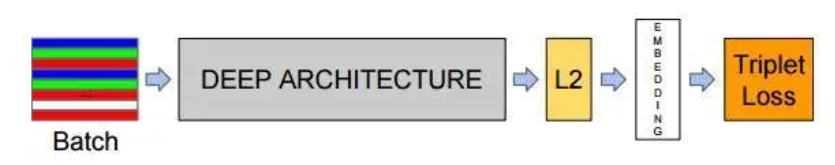
\includegraphics[width=0.7\textwidth]{FaceNet.png}
    \caption{FaceNet结构框架}
    \label{fig:FaceNet}
\end{figure}
,它以人脸图像作为输入,并通过多层卷积和池化操作,最终将输入图像映射到一个128维的向量空间中。在训练模型时采用了triplet\_loss(见图$\left(\ref{fig:TripletLoss}\right)$)来衡量训练过程中样本之间的距离误差,在这个损失函数中,每个训练样本由三个人脸图像组成:锚点人脸图像(Anchor Face)、正样本人脸图像(Positive Face)和负样本人脸图像(Negative Face)。模型的目标是使得锚点人脸图像与正样本人脸图像的距离尽可能小,与负样本人脸图像的距离尽可能大,从而使得人脸嵌入在向量空间中能够很好地区分不同的人脸。简言之,在训练前或者在线学习中不断给神经网络制造“困难”,即一直在寻找与样本最不像的“自己”,同时寻找与自己最像的“他人”。通过随机梯度下降法,不断缩短自身所有样本的差距,同时尽可能拉大与其他人的差距,最终达到一个最优。通过这样一种嵌入学习(Embedding learing),能对原始的特征提取网络输出层再进一步学习,从而改善特征的表达。
\begin{figure}[!ht]
    \centering
    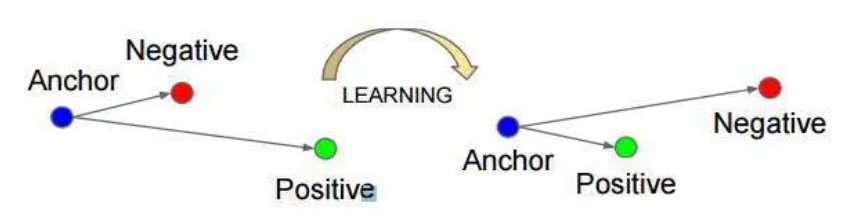
\includegraphics[width=0.7\textwidth]{TripletLoss.png}
    \caption{Triplet-Loss}
    \label{fig:TripletLoss}
\end{figure}

\begin{figure}[!ht]
    \centering
    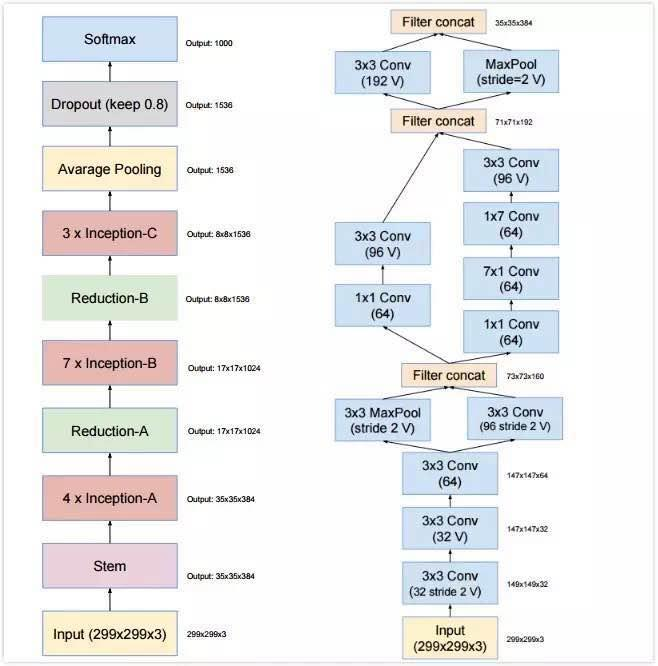
\includegraphics[width=0.5\textwidth]{InceptionResNetv2.jpg}
    \caption{Inception-ResNet-v2网络简化示意图}
    \label{fig:InceptionResNetv2}
\end{figure}

对于整个FaceNet结构,这里的特征提取可以当作一个黑盒子,可以采用各式各样的网络。最早的FaceNet采用两种深度卷积网络:经典Zeiler\&Fergus架构和Google的Inception v1。最新的FaceNet进行了改进,主体模型采用一个极深度网络Inception-ResNet-v2(见图$\left(\ref{fig:InceptionResNetv2}\right)$),由3个带有残差连接的Inception模块和1个Inception v4模块组成。


\subsubsection{中期设计}
我们中期使用的模型为基于VGG-face数据集预训练的ResNet50模型作为基础模型,并借助Keras深度学习框架构建了孪生神经网络结构。在模型构建过程中,我们去除了原始模型的输出层,保留了特征提取层,并设计了自定义的输出层模型,最终采用sigmoid层作为输出。这一设计旨在通过迁移学习,充分利用已有模型在大规模数据集上学习到的特征表达能力,从而提高模型的判断准确度。我们的目标是通过人脸图像进行血缘关系的判断,因此模型的输出层需要能够有效地区分不同人脸图像之间的相似度。采用孪生神经网络结构,可以使模型在学习过程中更好地捕捉到人脸图像之间的相似性特征,从而实现更精准的血缘关系判断。
\begin{enumerate}
    \item ResNet50模型
  
    ResNet50是ResNet系列中的一个特例,它有50层深,并且采用了残差模块的结构,克服了深度神经网络训练过程中的梯度消失和梯度爆炸等问题。通过使用残差连接,ResNet50模型使得神经网络可以更深更广地构建,从而在图像识别等任务中取得了更好的性能。
  
    ResNet50模型的结构相对简单,主要由一系列的残差模块组成,其中包括了卷积层、批量归一化层和激活函数。整个网络的结构可以分为预处理层、卷积层、全局平均池化层和全连接层几个部分。具体结构见图$\left(\ref{fig:ResNet50}\right)$
    \begin{figure}[!ht]
      \centering
      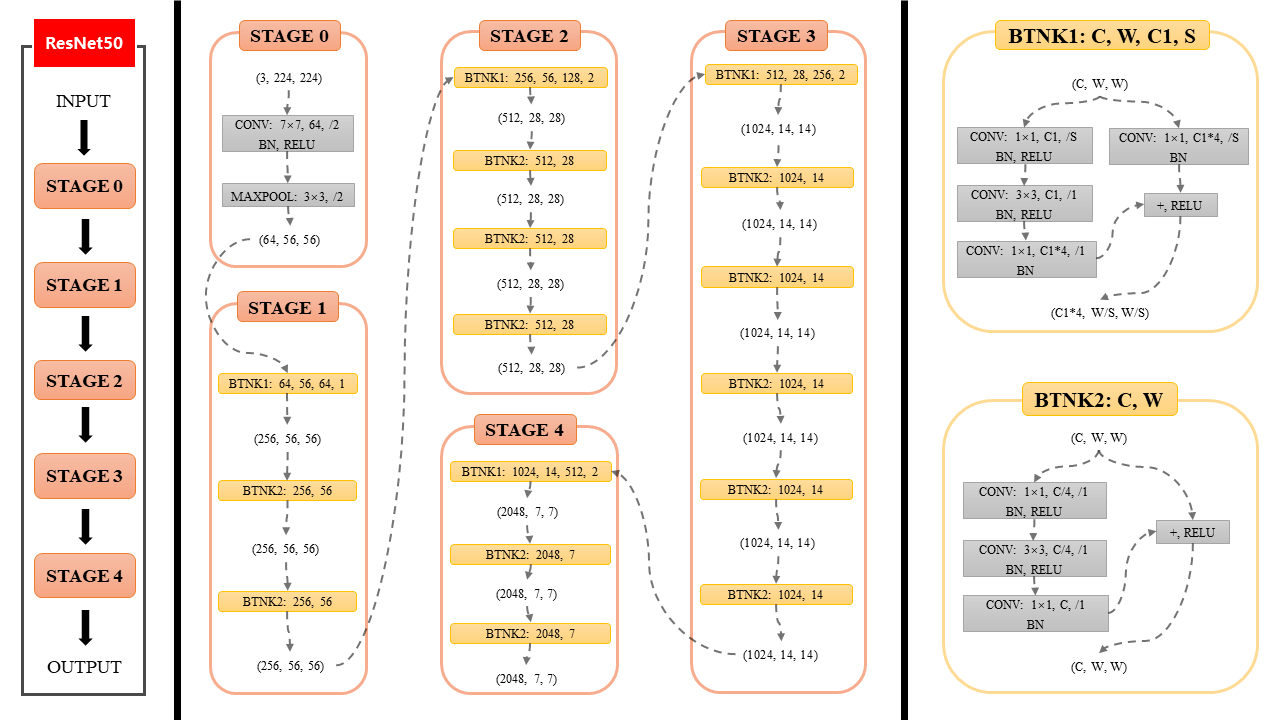
\includegraphics[width=0.7\textwidth]{ResNet50.png}
      \caption{ResNet50结构}
      \label{fig:ResNet50}
    \end{figure}

    \item 孪生神经网络
    
    孪生神经网络(Siamese Neural Network)是一种特殊的神经网络架构,最初用于解决用于度量学习(Metric Learning)的问题。孪生神经网络由两个完全相同的子网络组成,它们共享相同的权重和参数。这两个子网络被称为"孪生网络",因此得名"孪生神经网络"。
  
    孪生神经网络有两个输入(Input1 and Input2),将两个输入feed进入两个神经网络(Network1 and Network2),这两个神经网络分别将输入映射到新的空间,形成输入在新的空间中的表示。通过Loss的计算,评价两个输入的相似度。(详见图$\left(\ref{fig:Siamese network}\right)$)
    \begin{figure}[!ht]
      \centering
      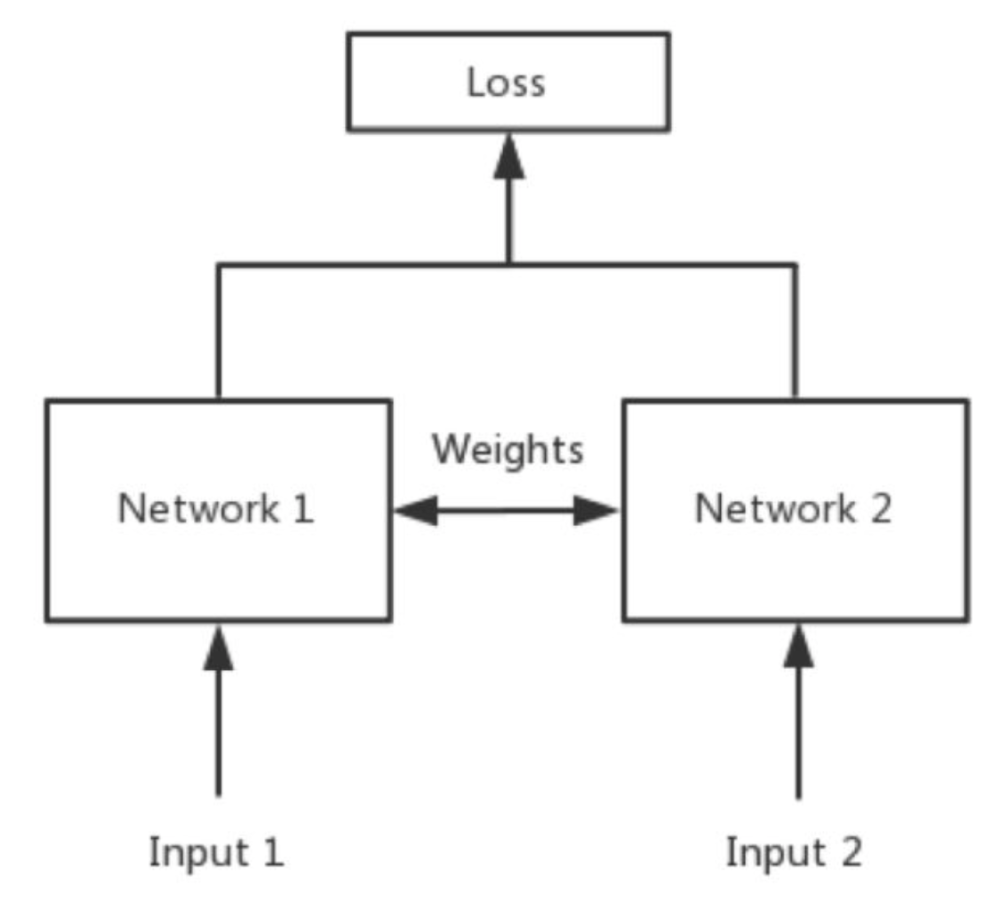
\includegraphics[width=0.7\textwidth]{Siamese network.png}
      \caption{Siamese network}
      \label{fig:Siamese network}
    \end{figure}
\end{enumerate}

在训练ResNet50模型时,首先,我们划分了训练数据集train\_images和验证数据集val\_images,
(见图$\left(\ref{fig:divide1}\right)$)
\begin{figure}[!ht]
  \centering
  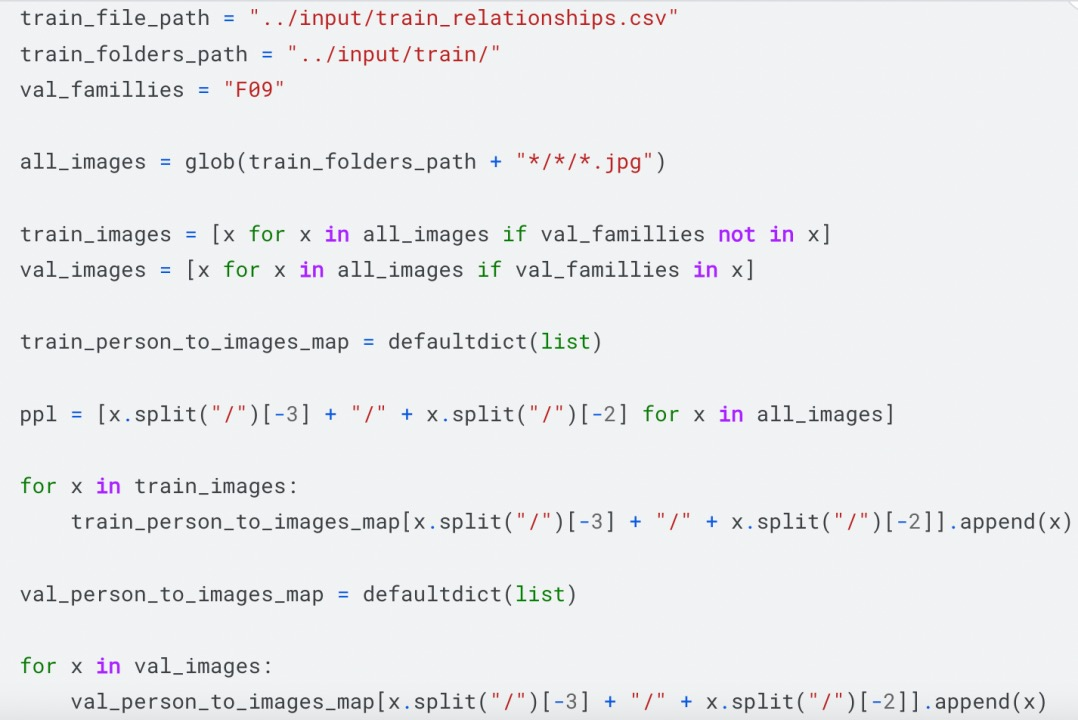
\includegraphics[width=0.5\textwidth]{divide.jpg}
  \label{fig:divide}
\end{figure}
\begin{figure}[!ht]
  \centering
  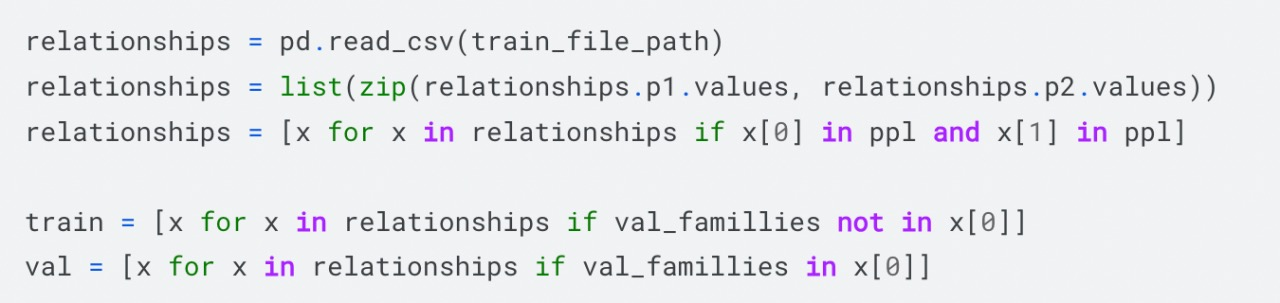
\includegraphics[width=0.5\textwidth]{divide1.jpg}
  \caption{划分训练数据集和验证数据集}
  \label{fig:divide1}
\end{figure}
接下来我们定义一个用于读取图片的函数,该函数需采用已经封装好的preprocess\_input函数。此外,我们还定义了一个生成器,这个生成器的作用是生成训练样本和测试样本。并且要设定相同的正负样本数。通过使用yield语句,能够在迭代的过程当中动态地生成数值。这种方式尤其适用于存在大量数据的情形,它能够助力节省内存空间。

\begin{figure}[!ht]
  \centering
  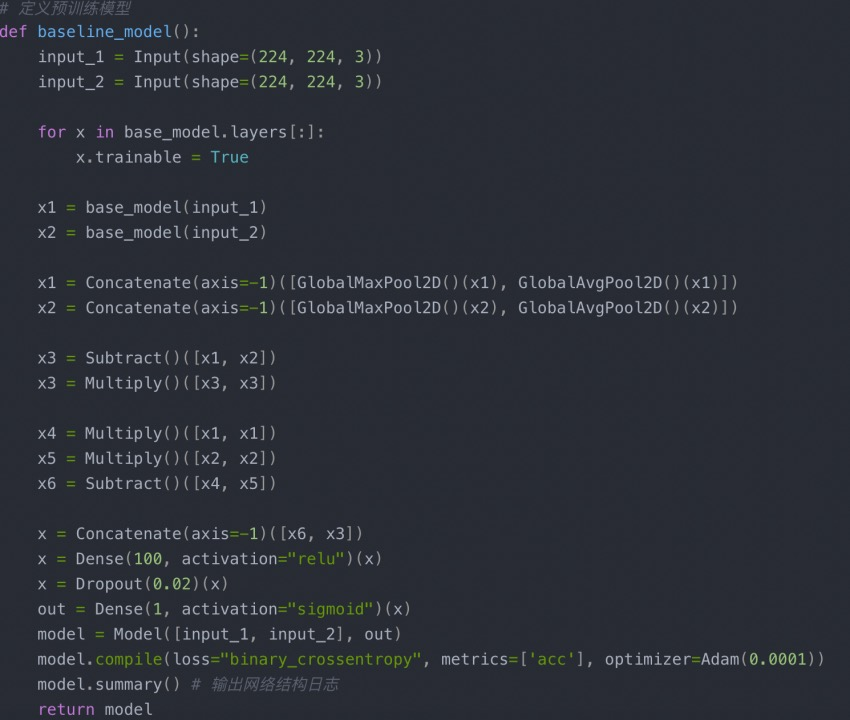
\includegraphics[width=0.7\textwidth]{model.jpg}
  \caption{模型定义}
  \label{fig:model}
\end{figure}
下面载入源自VGG-face数据集预训练的ResNet50模型,进而对模型予以定义。其基本思路为运用若干个Concatante层,之所以如此,是因为并不知晓哪种池化方法更为适宜,也不明确池化后的特征相乘后做差的效果更好,还是做差后相乘的效果更优,故而将这几种处理方式径直进行连接,交由网络自行学习。并采用二元交叉熵充当损失函数。该步骤的具体代码见图$\left(\ref{fig:model}\right)$。

然后我们定义了回调函数,用于保存模型和辅助模型训练,以及进行学习率的设置,代码见图$\left(\ref{fig:func}\right)$
\begin{figure}[!ht]
  \centering
  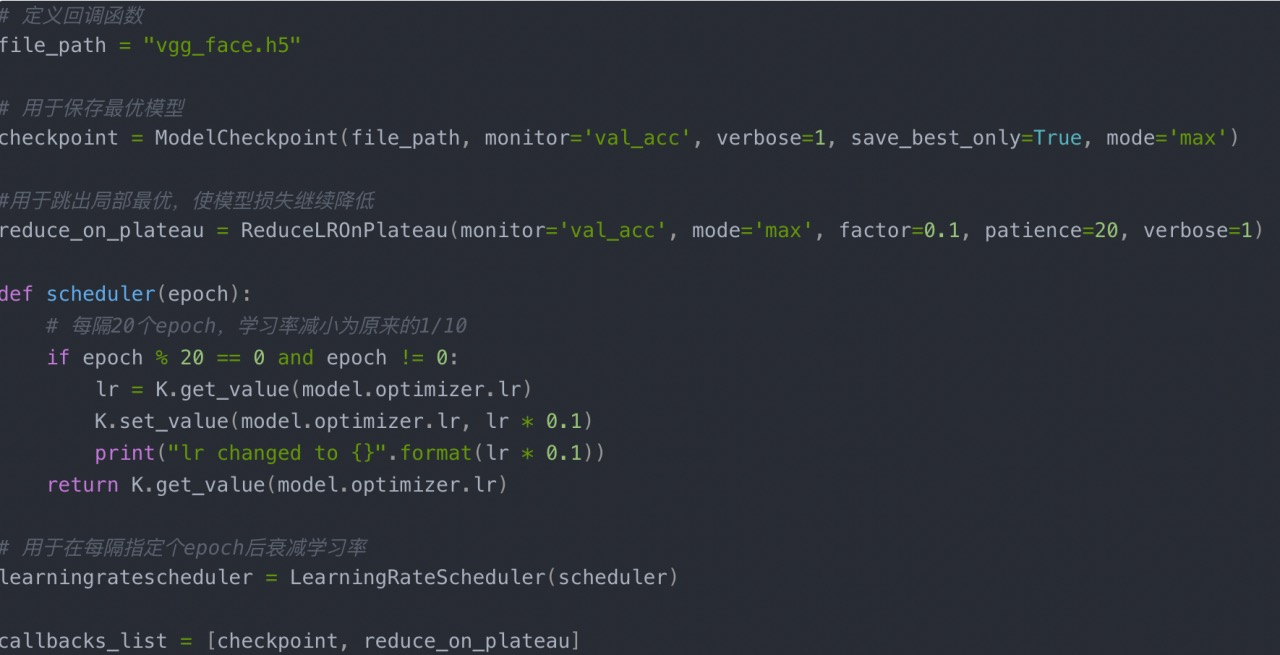
\includegraphics[width=0.7\textwidth]{func.jpg}
  \caption{回调函数}
  \label{fig:func}
\end{figure}

最后实施训练调参操作。首先将mode设置为‘train’,每个epoch迭代200次,总计训练100个epoch。待参数调好之后,再将mode设置为‘train\_valid’,运用全部的数据集重新展开训练,每个epoch迭代300次,同样训练100个epoch。

训练完成后,用该模型对测试集进行预测即可得到输出文件。

采用该模型,我们的得分Private Score为0.868,在Private 测试集上排名第189,Public Score为0.862,在Public测试集上排名第171(见图$\left(\ref{fig:scoremid}\right)$)。
\begin{figure}[!ht]
    \centering
    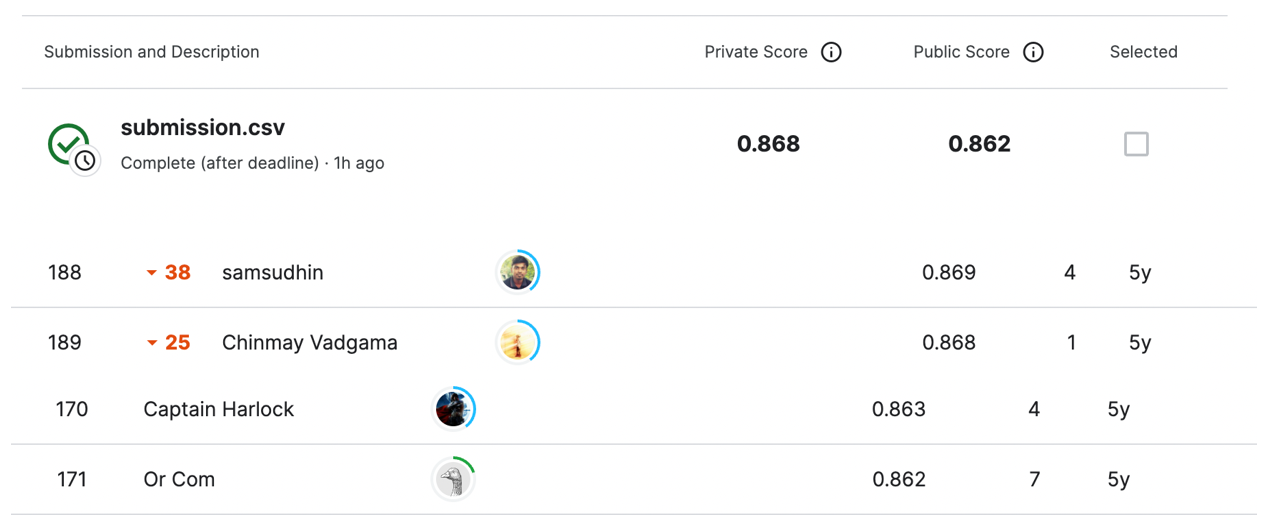
\includegraphics[width=0.7\textwidth]{scoremid.png}
    \caption{中期排名与结果}
    \label{fig:scoremid}
\end{figure}

\subsubsection{结题设计}
我们首先对中期的模型进行了修改,得到的模型识别正确率提升存在上限,但当我们浏览该比赛的讨论区时,发现排名靠前的队伍均使用了集成学习的思想。

集成学习通过结合多个基本模型的预测结果来提高模型的泛化能力和预测准确性。它通过将多个模型的预测结果进行加权平均、投票或者使用其他组合方法来做出最终的预测。集成学习的核心思想是“三个臭皮匠赛过诸葛亮”,即通过结合多个模型的优势来弥补单个模型的缺陷,从而获得更好的性能。

常见的集成学习方法包括:
\begin{enumerate}
  \item \textbf{Bagging(自举汇聚法)}
  
  通过随机采样训练数据集的子集来训练多个基学习器,然后将它们的预测结果进行平均或投票来得到最终的预测结果。常见的算法包括随机森林(Random Forest)。自举汇聚法可以降低模型的方差,提高模型的稳定性和泛化能力。还能减少过拟合的风险,因为每个基学习器都是在不同的训练子集上训练得到的,减少了模型对训练数据的过度依赖。
  \begin{figure}[!ht]
    \centering
    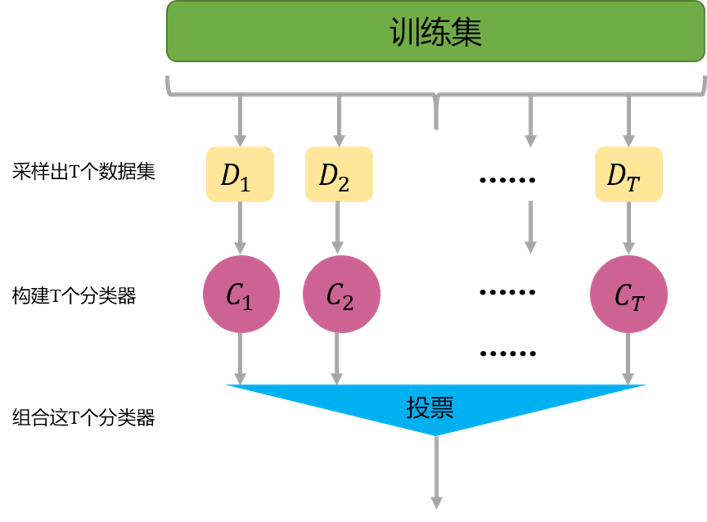
\includegraphics[width=0.5\textwidth]{bagging.png}
    \caption{自举汇聚法}
    \label{fig:bagging}
  \end{figure}
  \item \textbf{Boosting(提升法)}
  
  通过串行训练多个基学习器,每个基学习器都试图修正前一个学习器的错误,从而逐步提升模型性能。常见的算法包括AdaBoost、Gradient Boosting等。提升法的核心是在每一轮迭代中,通过调整样本的权重或者基学习器的权重,使得模型在前一轮中被错误分类的样本在下一轮中得到更多的关注,从而逐步减少模型的偏差。提升法在实际应用中被广泛使用,尤其在分类和回归问题中表现出色,能够处理复杂的非线性关系和高维数据集,并且具有很强的泛化能力。
  \begin{figure}[!ht]
    \centering
    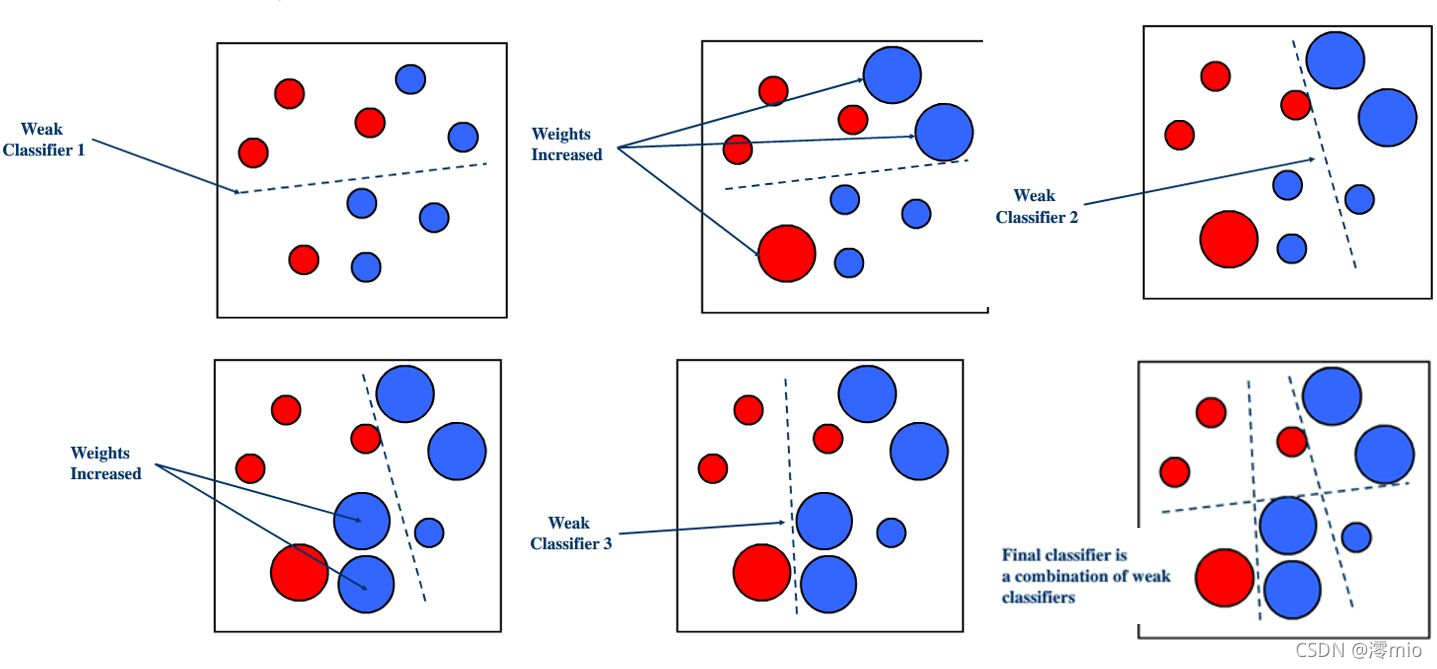
\includegraphics[width=0.5\textwidth]{boosting.png}
    \caption{提升法}
    \label{fig:boosting}
  \end{figure}
  \item \textbf{Stacking(堆叠法)}
  
  将多个不同的基学习器的预测结果作为新的训练数据,然后训练一个元学习器(或称为组合模型)来预测最终的输出。堆叠法能够充分利用不同类型的基学习器的优势,提高模型的泛化能力和预测性能。也可以有效地减少过拟合的风险,因为元学习器通常是在一个新的特征空间上进行训练,而不是直接在原始数据上进行训练。但堆叠法的训练过程相对复杂,需要进行多轮的训练和预测,可能会增加模型的计算复杂度和内存消耗。
  \begin{figure}[!ht]
    \centering
    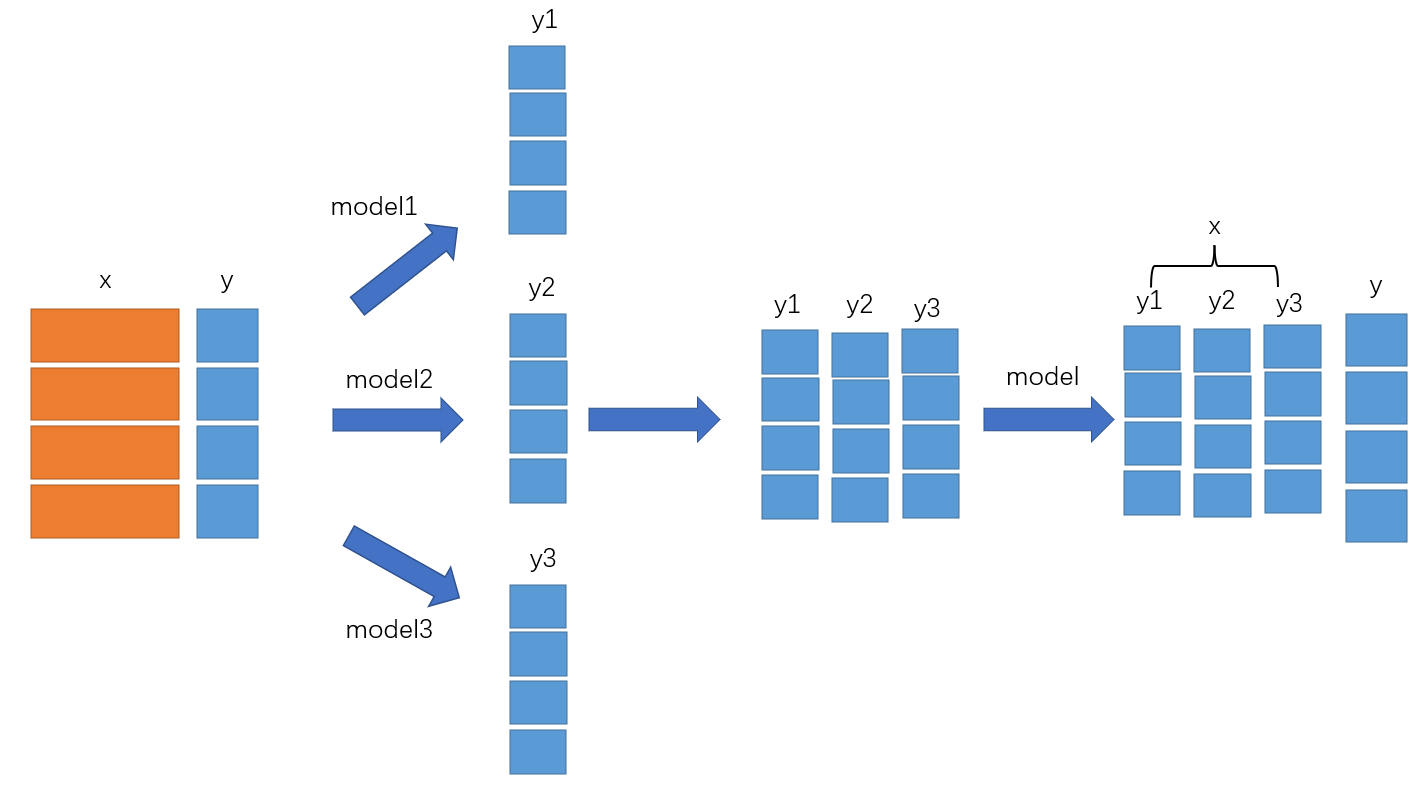
\includegraphics[width=0.5\textwidth]{stacking.png}
    \caption{堆叠法}
    \label{fig:stacking}
  \end{figure}
\end{enumerate}


\subsection{结题最终结果分析}
我们在中期使用的ResNet50模型基础上增加了FaceNet模型一起用来提取特征,使提取出的特征更加全面,同时增加了新的特征处理方式,具体过程如下:
\begin{itemize}
  \item 进行图像预处理并且定义生成器函数,代码如图$\left(\ref{fig:getfeature}\right)$所示
  \begin{figure}[!ht]
    \centering
    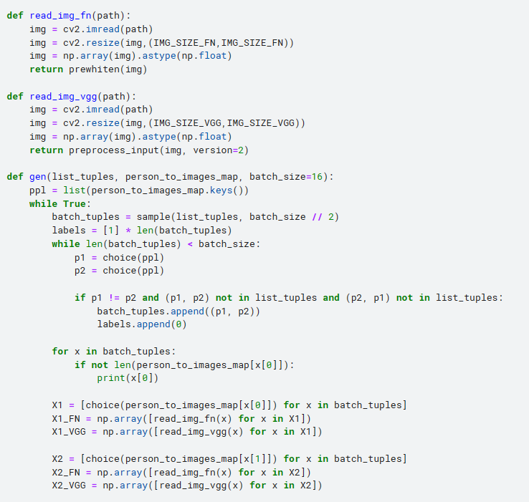
\includegraphics[width=0.7\textwidth]{getfeature.png}
    \caption{图像预处理与生成器函数}
    \label{fig:getfeature}
  \end{figure}
  \item 结合ResNet50模型和FaceNet模型的识别结果,将ResNet50模型得到的特征向量存储至$x_1$与$x_2$中,将FaceNet模型得到的特征向量存储至$x_3$与$x_4$中,并对特征向量进行$x_1+x_2$、$x_3+x_4$、$x_1-x_2$、$x_3-x_4$、$x_1\cdot x_2$、$x_3\cdot x_4$、$x_1^2+x_2^2$、$x_3^2+x_4^2$的一系列操作。代码如图$\left(\ref{fig:feature}\right)$所示
  \begin{figure}[!ht]
    \centering
    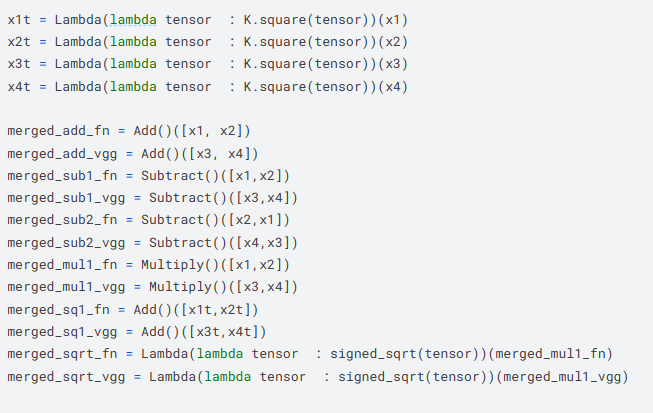
\includegraphics[width=0.7\textwidth]{feature.png}
    \caption{处理特征向量}
    \label{fig:feature}
  \end{figure}
  \item 将上述处理过后的特征向量合成为一个向量,以进行特征的融合。将合成后的向量输入至激活函数ReLu中,对特征进行线性变换和非线性映射,以增加模型的表达能力。然后在Dropout层中随机丢弃10\%的神经元,以减少过拟合。减少密集连接层的单元数量,重复上述操作,最后在具有单个单元的密集连接层,使用 sigmoid 激活函数得到最终的位于0,1区间内的概率值。代码如图$\left(\ref{fig:output}\right)$所示
  \begin{figure}[!ht]
    \centering
    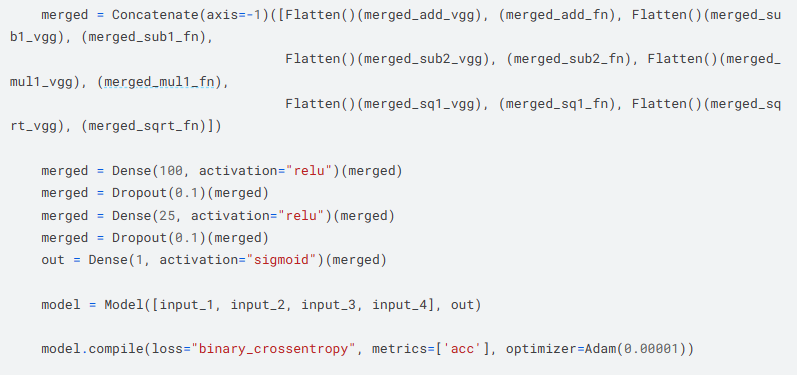
\includegraphics[width=0.7\textwidth]{output.png}
    \caption{神经网络的建立与结果输出}
    \label{fig:output}
  \end{figure}
\end{itemize}

最终得到的结果在得分上有着显著的提升(详见图$\left(\ref{fig:improve}\right)$)
\begin{figure}[!ht]
  \centering
  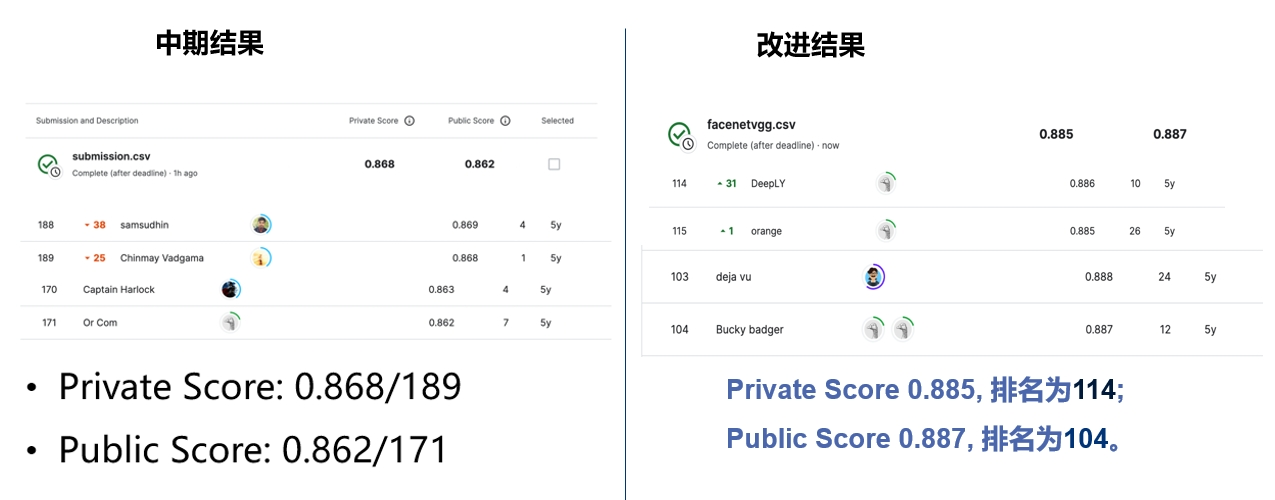
\includegraphics[width=0.6\textwidth]{improve.png}
  \caption{中期结果加入FaceNet模型后的提升}
  \label{fig:improve}
\end{figure}

如上文所述,我们浏览了该比赛的讨论区,发现排名靠前的队伍均使用了集成学习的思想,于是我们参考集成学习的思想,重新定义了四个模型(使用不同的特征提取模型、更改特征处理方式等),再分别对这四个模型进行如上所述的训练,使用训练好的模型对结果进行预测并提交,观察该模型预测结果的得分,通过公式$y=\sum_{i = 1}^{5} w_ix_i $加权处理,得分高的取较高权重$w_i$,并再次将加权处理后的结果提交,观察得分是否变高,若变高,则将此次提交的文件置换原有公式中分数较低的那个文件,并重新分配权重$w_i$,再次得到新的预测结果,如此往复进行递归操作,当分数不再提高时停止。最终得到的结果在Private测试集上的得分为0.918, 排名第5;在Public测试集上的得分为0.914, 排名第6。

经我们分析,能获得极大提升的原因如下:
\begin{enumerate}
  \item \textbf{提升了模型的多样性}:以FaceNet模型和ResNet50模型为例,FaceNet模型主要侧重于人脸特征的提取和表示,而ResNet50模型是一个通用的图像分类模型,这两种模型是不同的,它们具有不同的架构和特征表示能力。通过将它们集成在一起,可以增加模型的多样性,模型能够学习到更丰富的图像特征,从而提高模型的泛化能力。
  \item \textbf{模型间的错误互相补偿}:由于FaceNet模型和ResNet50模型是两个不同的模型,它们可能会在不同的样本上产生不同的错误。通过将它们的预测结果进行加权平均或投票,可以减少错误的累积,从而提高模型的整体性能。
  \item \textbf{降低了过拟合风险}:集成学习可以降低模型的方差,减少过拟合的风险。FaceNet模型和ResNet50模型可能在不同的数据子集上表现更好,通过集成学习可以有效地减少模型的方差,提高模型的稳定性和泛化能力。
  \item \textbf{提升了特征的丰富性}:FaceNet模型和ResNet50模型分别学习了人脸特征和图像特征,通过将它们的特征表示进行组合,可以得到更丰富和更具区分性的特征表示,从而提高了模型的识别性能。
\end{enumerate}

\subsection{结题主要问题分析}
在我们训练模型的过程中,主要遇见了以下问题:
\begin{enumerate}
  \item \textbf{单一模型的识别能力存在上限}:无论我们怎么优化某一模型,其识别正确率总会存在上限,无法进一步地提高,识别正确率无法超过90\%。
  \item \textbf{图像的特征提取不充分}:在我们使用ResNet50模型进行图像特征的提取时,受该模型的特征提取器影响,可能会遗漏图像中人脸的特征,进而导致血缘关系判断的错误。
  \item \textbf{训练所用数据集质量不高}:官方给出的测试文件中的部分图片质量不高,有些存在大量噪点,有些人像的面部亮度不足,有些人像的面部被部分遮挡等等,这些因素都会导致我们所训练的模型识别正确率较低。
\end{enumerate}

我们对这些问题进行了分析,并得出了相应的解决措施:
\begin{enumerate}
  \item \textbf{采用集成学习的方式提升模型的泛化能力}:如上文所述,我们使用了五种模型得到的预测结果并对其进行加权处理,最终得到的预测结果相较单一模型有着很大的提升,不仅提高了我们的得分与排名,也使模型对图像人脸特征的提取更加充分。
  \item \textbf{对训练集进行数据预处理}:我们在训练模型前先对训练集中的图像进行了预处理,对图像进行白化处理,使所有图片的亮度均衡化;对部分图像进行颜色通道对齐处理,对其该图像的RGB通道,提升图片质量;使用Yolov5算法进行目标检测,识别脸部位置,便于人脸特征的提取。
\end{enumerate}

\section{结题后拟改进措施}
\subsection{增加新的特征提取模型}
在查找提取图片特征的模型时,我们注意到一个名为SENet50的图片特征提取模型,它结合了ResNet50和SE(Squeeze-and-Excitation)模块这样就可以在学习特征的同时,自适应地调整特征图的权重,提高了模型的性能。在SE模块中,它通过对特征通道进行重新校准来提高网络的表现,使得网络更加关注对分类任务有用的特征。

SE模块由两个步骤组成:压缩(Squeeze)和激励(Excitation):
\begin{enumerate}
  \item \textbf{压缩}:SE模块通过全局平均池化操作将输入的特征图压缩成一个特征向量,这个特征向量反映了每个通道的全局特征重要性。可通过公式
  \begin{gather}
    z_c=F_sq(u_c)=\frac{1}{H\times W}\sum_{i = 1}^{H} \sum_{i = 1}^{W} u_c(i,j)
  \end{gather}
  实现全局信息的获取。
  \item \textbf{激励}:特征向量经过一个全连接的神经网络,这个网络通常包括一个或多个全连接层,其输出是一个表示每个通道重要性的权重向量。这个权重向量通过 Sigmoid 激活函数进行归一化,然后被应用到输入的特征图上。Sigmoid 激活函数如下式
  \begin{multline}
     s=F_ex(z,W)=\sigma (W_2\delta (W_1z))\\
     where,W_1\in \mathbb{R}^{\frac{C}{r}\times C},W_2\in \mathbb{R}^{C\times\frac{C}{r} } 
  \end{multline}
\end{enumerate}
通过引入SENet50模型,也许能够从图片中提取出更优质的特征,以用于后续的集成学习。

\subsection{优化集成学习过程}
由于时间有限,我们没有花费过多的时间进行集成学习,这可能导致我们最终的提交结果并未收敛,也许仍存在最优解。后续会对集成学习过程进行优化,以找到最优的权重值。


\section{参与项目体会}
\begin{itemize}
  \item \textbf{刘**}:
  
  在本次挑战课程的学习中,我实属收益颇丰。在理论课程中,我学到了近乎全面的人工智能领域理论知识,在实验课与 kaggle 项目中 中,我也运用了诸多人工智能的算法。

  在近两年如火如荼的人工智能狂潮中,我也借此课程的机会,开始了人工智能方面的学习。通过本次 kaggle 项目-东北大学实验室提出的识别图像是否具有血缘关系项目,我们组使用了今几年较火诸如 FaceNet,   VGGFace 等模型,也借此理解了神经网络等架构的思想。

  在理论入门、算法复刻、数据分析、数据处理、模型构建、模型改进等诸多过程之后,我的理论知识和实践能力耶随之增强着。通过团队成员所有人的鼎力合作,积极沟通,我们最终以一个优秀的成绩完成了本次 kaggle 项目,实现了我们团队在学期初给自己定下的目标。
  
  同时,老师在项目推进中反复提到的整体与局部概念也令我们受益匪浅,相信日后该项目的经历以及思想的深入一定会对我们的学习有着更多的帮助。
  \item \textbf{赵**}:
  
  本次挑战课中,我接触了机器学习的相关知识,了解了人工智能背后的专业知识,学会了如何训练自己的神经网络模型。在项目进行的过程中,我主要负责论文的编写以及PPT的制作,这使我掌握了\LaTeX 这门非所见即所得的文章排版语言的使用,使用\LaTeX 编写生成的文章排版及其工整,令人赏心悦目。除此之外,在对模型进行集成学习训练时,我也深谙“三个臭皮匠赛过诸葛亮”的道理,使我明白了团队合作的重要性。
  \item \textbf{武**}:
  
  参与这次项目对我来说帮助真的很大,不同于以往别的只重理论教学的课程,这次的人工智能课程给了我一次很好的实战机会,让我真切的感受到人工智能的应用。从完全没接触过人工智能,到结课时却能较熟练地搭建一个项目,这其中的成长是显而易见的。借助我们所选的这个血缘关系识别的项目,从eda开始,我们不断探索不同的模型与处理,从facenet到resnet再到两者的结合以及最后集成学习的使用,我不仅学会了如何运用Facenet和ResNet等模型进行人脸识别和血缘关系判断,还深刻领悟到了集成学习的力量,虽然计算成本翻倍提高,但所带来的效果确是十分强大的。在团队合作的过程中,我也学到了如何进行团队合作,明确各方需求和意见,让团队朝着共同的目标努力。我们每个人都充满了热情和专业精神,我们在挑战中共同成长,最终取得了令人满意的成绩。这段经历将成为我宝贵的回忆,感谢我的团队成员,感谢老师。
  \end{itemize}


\section{意见与建议}
\begin{enumerate}
  \item \textbf{课堂讲授内容由浅入深}:人工智能与机器学习毕竟存在着一定的技术门槛,尤其对于大二编程基础不够扎实的我们来说难度与挑战很大,希望老师能在开始的几节课上加入一些示例代码的讲解,带领我们快速入门。
  \item \textbf{实验指导书内容详细化}:在做实验的过程中,我们发现实验指导书中的部分内容在理解上存在困难,导致实验进展缓慢,希望实验指导书中的实验步骤部分能够更加详细,便于实验的完成。
  \item \textbf{课堂展示形式多样化}:在课堂上进行小组成果展示时,没有轮到的小组参与度不高,课堂互动率较低,希望可以增加课堂互动形式,提高同学们的参与度。
\end{enumerate}


\newpage

\begin{thebibliography}{99}
  \bibitem{1} Florian Schroff, Dmitry Kalenichenko, James Philbin. FaceNet: A Unified Embedding for Face Recognition and Clustering. In Proceedings of the IEEE conference on computer vision and pattern recognition (CVPR), pages 815–823, 2015.
  \bibitem{2} Kaiming He, Xiangyu Zhang, Shaoqing Ren, and Jian Sun. Deep residual learning for image recognition. In Proceedings of the IEEE conference on computer vision and pattern recognition (CVPR), pages 770–778, 2016.
  \bibitem{3} Yaniv Taigman, Ming Yang, Marc'Aurelio Ranzato, and Lior Wolf. Deepface: Closing the gap to human-level performance in face verification. In Proceedings of the IEEE conference on computer vision and pattern recognition (CVPR), pages 1701–1708, 2014.
  \bibitem{4} Jerome H. Friedman. Greedy function approximation: A gradient boosting machine. Annals of Statistics, 29(5):1189-1232, 2001.
  \bibitem{5} Tianqi Chen and Carlos Guestrin. XGBoost: A Scalable Tree Boosting System. In Proceedings of the 22nd ACM SIGKDD International Conference on Knowledge Discovery and Data Mining, pages 785–794, 2016.
  \bibitem{6} Amit Dhurandhar, Akshay Gadi Patil, Prithwijit Guha, and Ganesh Ramakrishnan. DeepMEMNet: A deep learning framework for pan-specific MHC class I peptide binding prediction. BMC Genomics, 20(Suppl 2):165, 2019.
  \bibitem{7} Zagoruyko, S., \& Komodakis, N. (2015). Learning to compare image patches via convolutional neural networks. In Proceedings of the IEEE conference on computer vision and pattern recognition.
  \bibitem{8} Deng, J., Dong, W., Socher, R., Li, L. J., Li, K., \& Fei-Fei, L. (2009). ImageNet: A large-scale hierarchical image database. In 2009 IEEE conference on computer vision and pattern recognition.
  \bibitem{9} Koch, G., Zemel, R., \& Salakhutdinov, R. (2015). Siamese Neural Networks for One-shot Image Recognition. In Proceedings of the 32nd International Conference on Machine Learning (ICML) (Vol. 37, pp. 1774-1782).
  \bibitem{10} Taigman, Y., Yang, M., Ranzato, M., \& Wolf, L. (2014). DeepFace: Closing the Gap to Human-Level Performance in Face Verification. In Proceedings of the IEEE Conference on Computer Vision and Pattern Recognition (CVPR) (pp. 1701-1708).
\end{thebibliography}
\end{document}